\textbf{Wonder3D}~--~This method operates by leveraging a Domain Switcher technique when provided with an image. It produces color images and normal maps from multiple viewpoints of the given image, ensuring consistency across these views. This approach is pivotal for obtaining a comprehensive understanding of the model, not just from the front perspective but from all angles. In this particular test, the same input image as used for Magic123 was employed, which can be viewed in Figure~\ref{fig:inputAndModel} part (b). Figure~\ref{fig:initializationWonder3D} in the appendix illustrates the six viewpoints generated by Wonder3D, including front, front-right, right, back, left, and front-left views, each accompanied by its respective normal maps and color images. Utilizing these outputs, the model strives to construct a coherent and consistent 3D representation.

Contrasting with other methods, Wonder3D does not currently provide detailed validation images throughout the training process. Instead, outputs are available only at intervals of every 3000 iterations, as depicted in Figure~\ref{fig:generationWonder3D}. Without the ability to identify the relevant part of the original code to change this interval, progress can only be observed through these less frequent updates. From the available images, it is observed that the improvements in the model, based on the initially generated normals and color images, are relatively minor over the course of 10000 iterations. These slight enhancements are manifested in modest improvements in detail and the overall shape of the model, but they do not represent significant advancements from the initial stages.

\begin{figure}[H]
    \centering
    \begin{subfigure}[b]{0.18\textwidth}
        \centering
        \fontsize{9pt}{7pt}\selectfont\text{Iteration = 0}
        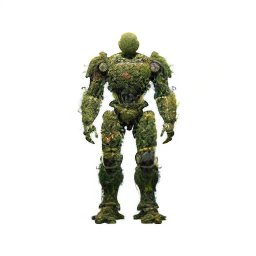
\includegraphics[width=\textwidth]{etc/a robot made out of plants/wonder3d/rgb_000_front}
        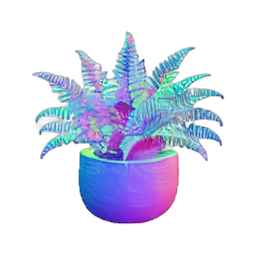
\includegraphics[width=\textwidth]{etc/a robot made out of plants/wonder3d/normals_000_front}
        \caption{}
    \end{subfigure}
    \begin{subfigure}[b]{0.18\textwidth}
        \centering
        \fontsize{9pt}{7pt}\selectfont\text{Iteration = 3000}
        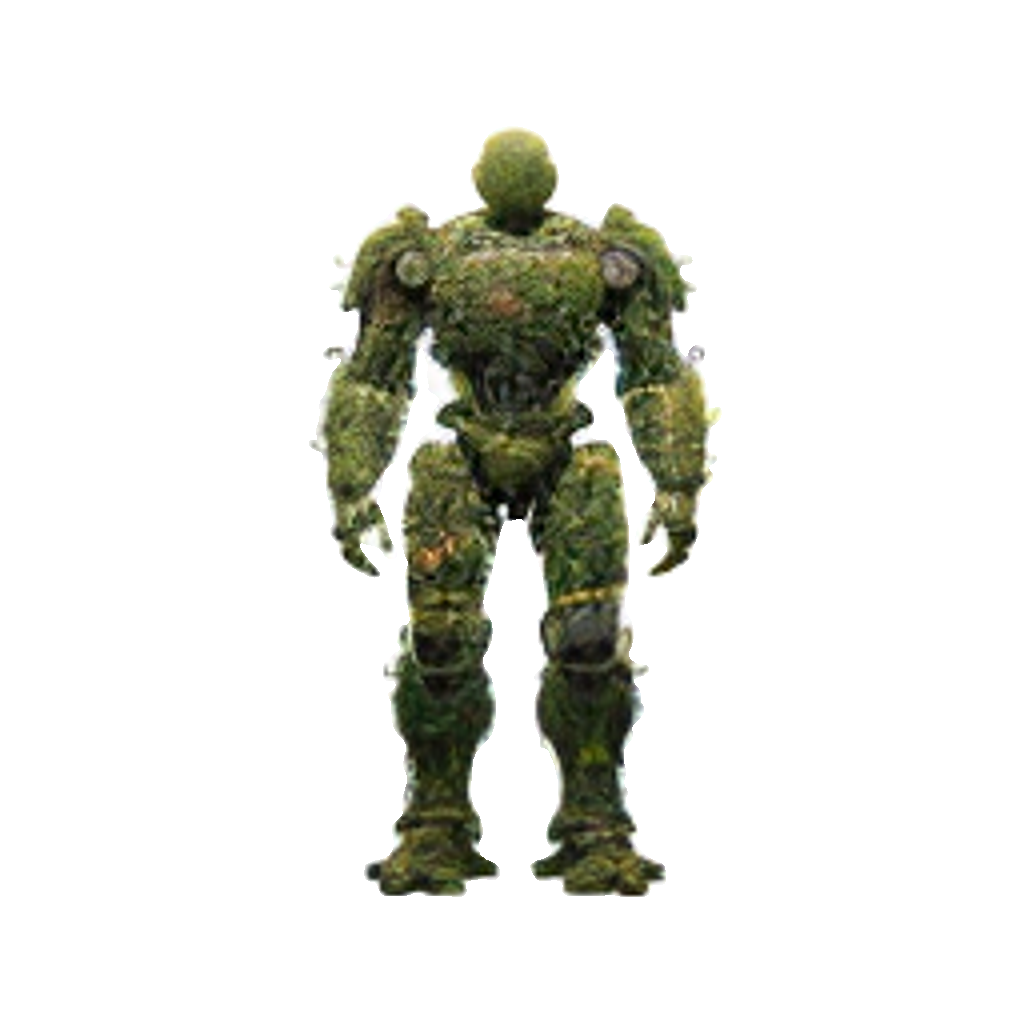
\includegraphics[width=\textwidth]{etc/a robot made out of plants/wonder3d/test/wonder3D_3000_front_part1}
        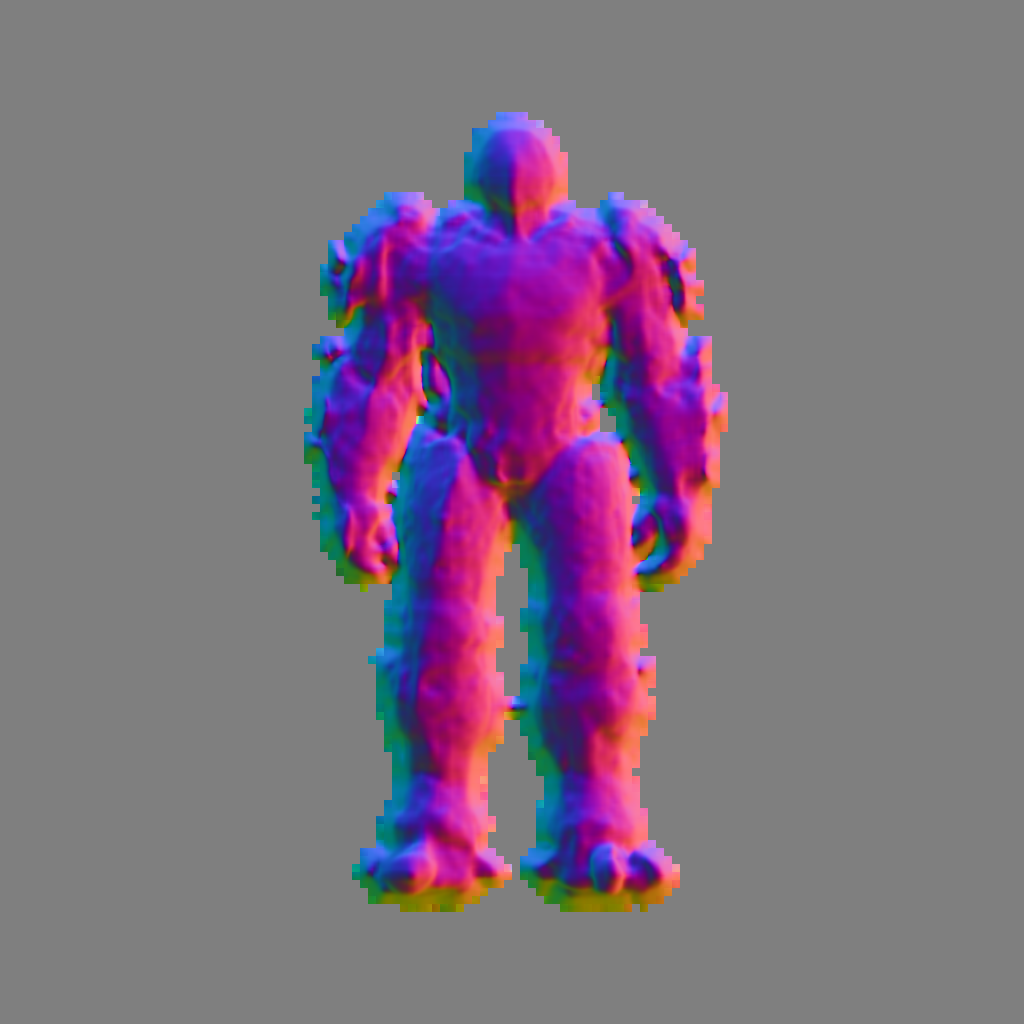
\includegraphics[width=\textwidth]{etc/a robot made out of plants/wonder3d/test/wonder3D_3000_front_part4}
        \caption{}
    \end{subfigure}
    \begin{subfigure}[b]{0.18\textwidth}
        \centering
        \fontsize{9pt}{7pt}\selectfont\text{Iteration = 6000}
        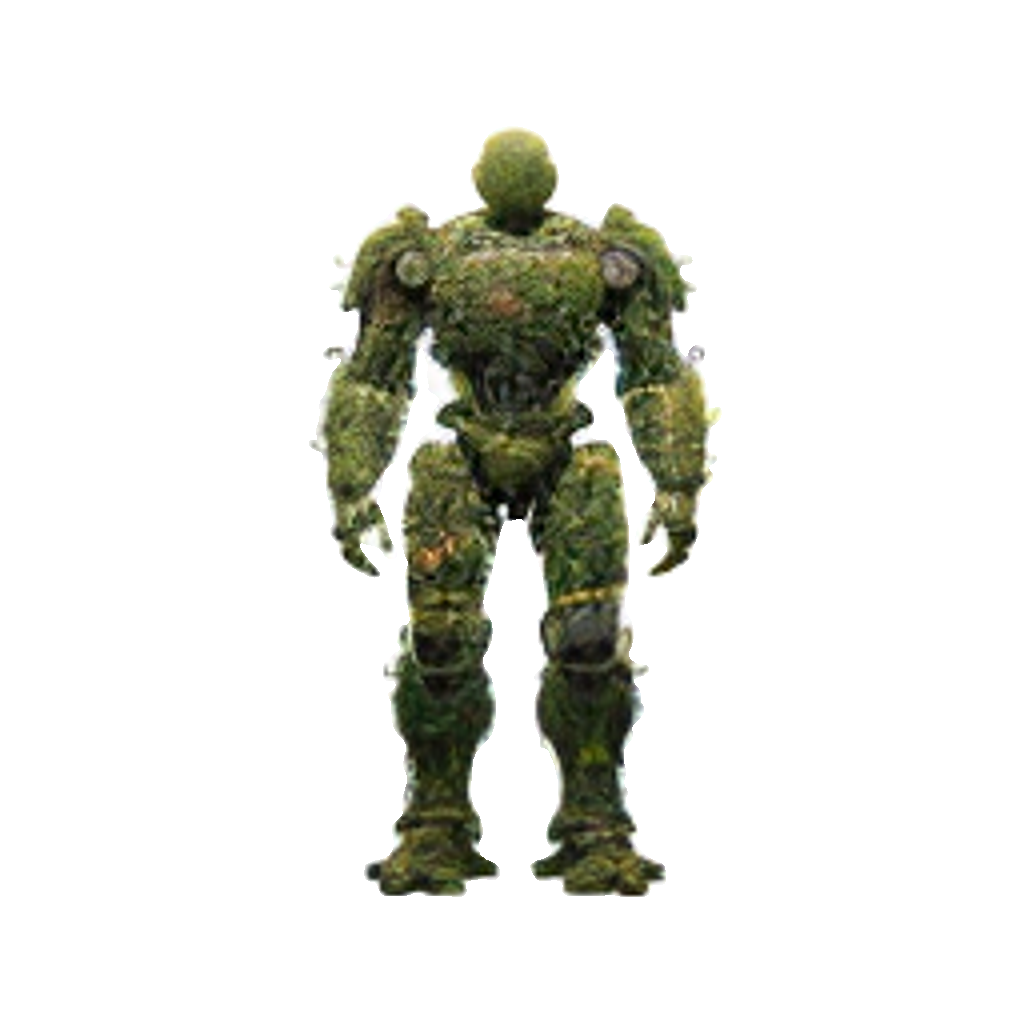
\includegraphics[width=\textwidth]{etc/a robot made out of plants/wonder3d/test/wonder3D_6000_front_part1}
        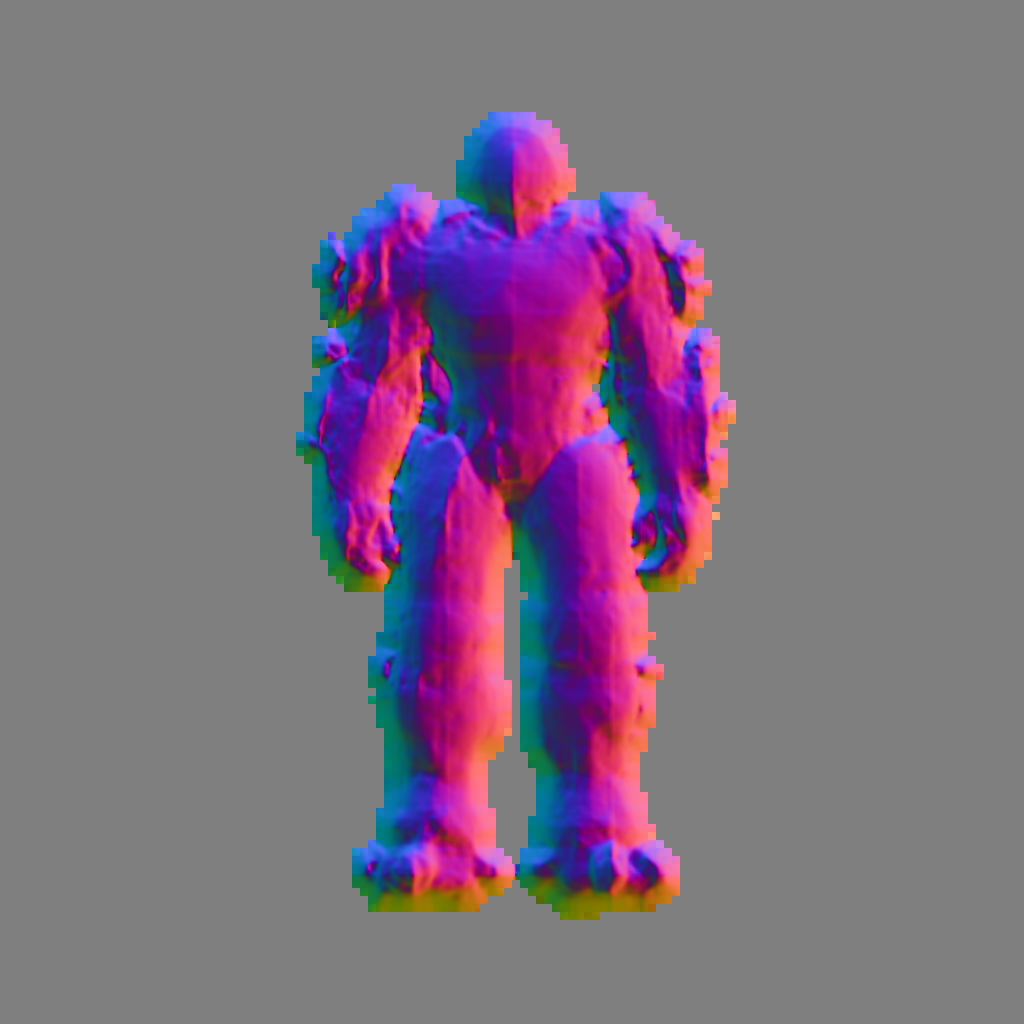
\includegraphics[width=\textwidth]{etc/a robot made out of plants/wonder3d/test/wonder3D_6000_front_part4}
        \caption{}
    \end{subfigure}
    \begin{subfigure}[b]{0.18\textwidth}
        \centering
        \fontsize{9pt}{7pt}\selectfont\text{Iteration = 9000}
        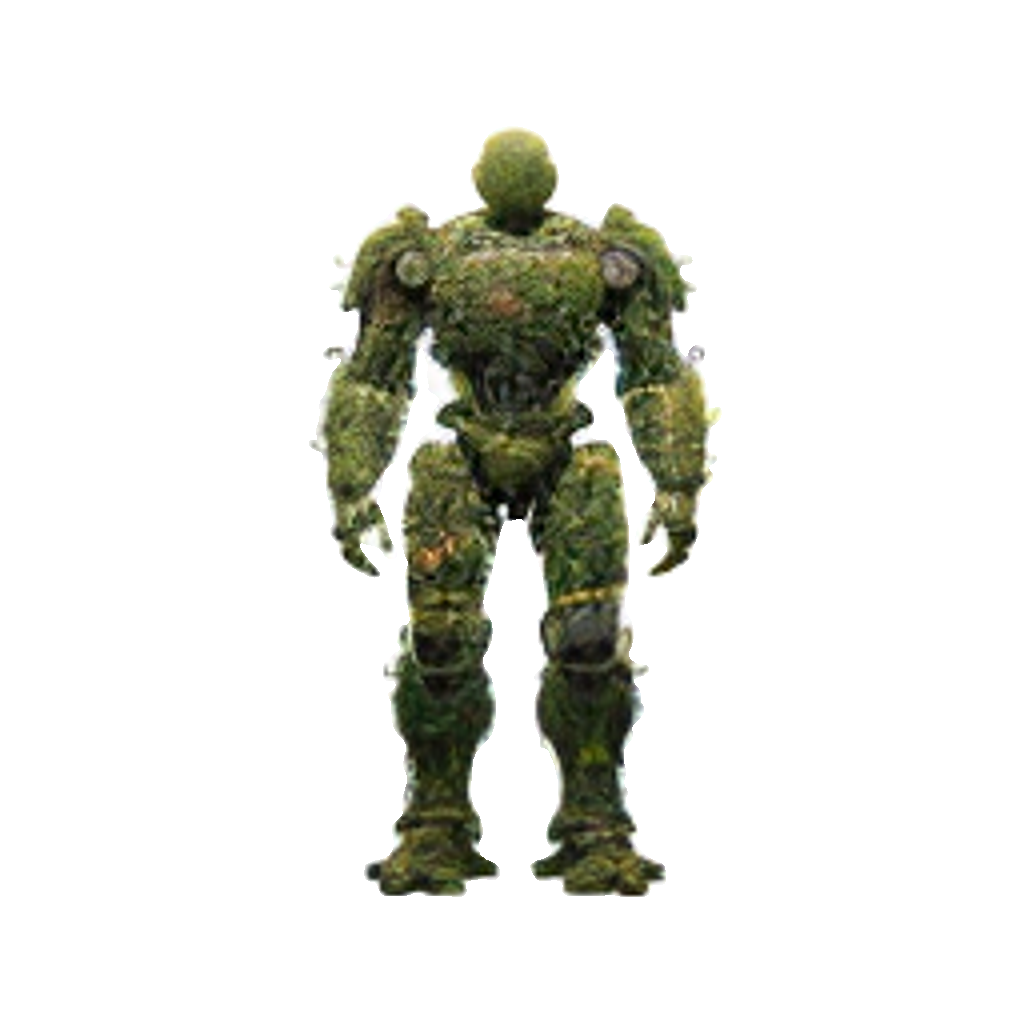
\includegraphics[width=\textwidth]{etc/a robot made out of plants/wonder3d/test/wonder3D_9000_front_part1}
        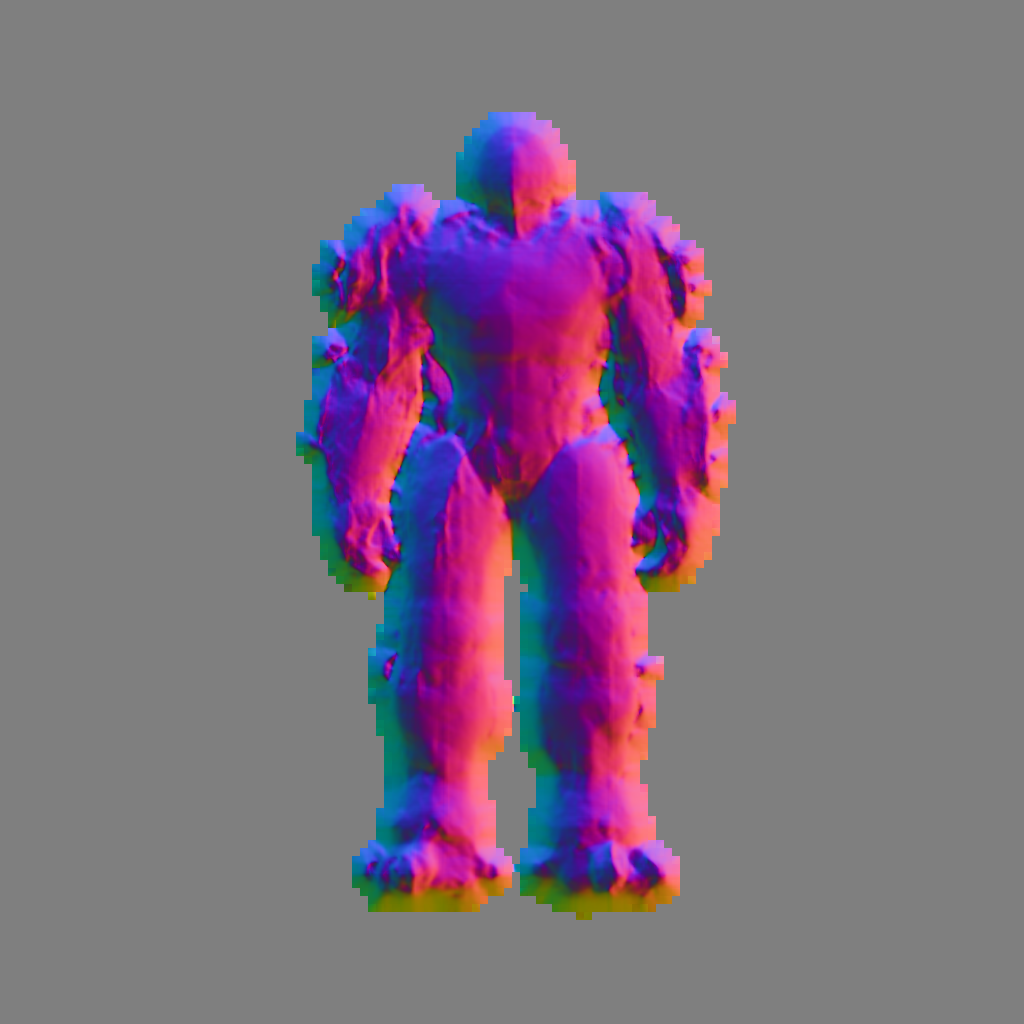
\includegraphics[width=\textwidth]{etc/a robot made out of plants/wonder3d/test/wonder3D_9000_front_part4}
        \caption{}
    \end{subfigure}
    \begin{subfigure}[b]{0.18\textwidth}
        \centering
        \fontsize{9pt}{7pt}\selectfont\text{Iteration = 10000}
        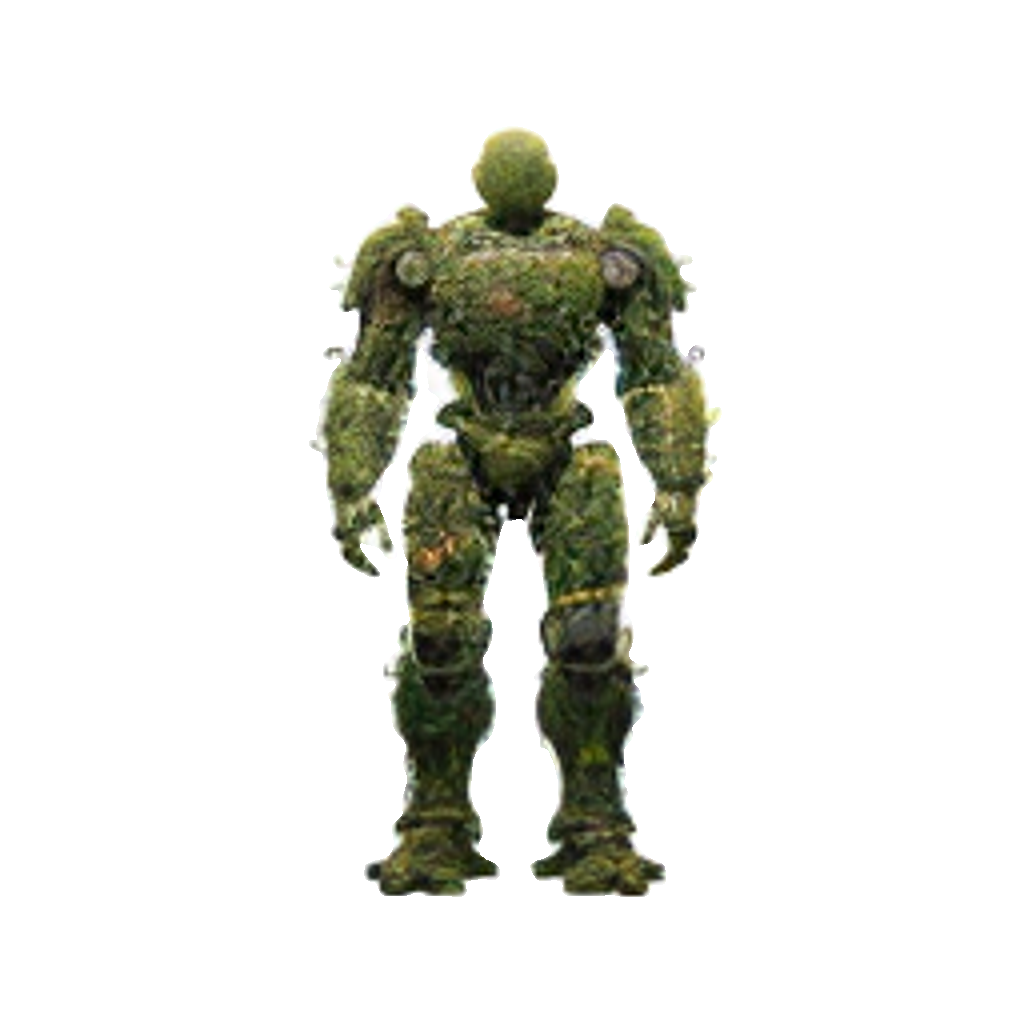
\includegraphics[width=\textwidth]{etc/a robot made out of plants/wonder3d/test/wonder3D_10000_front_part1}
        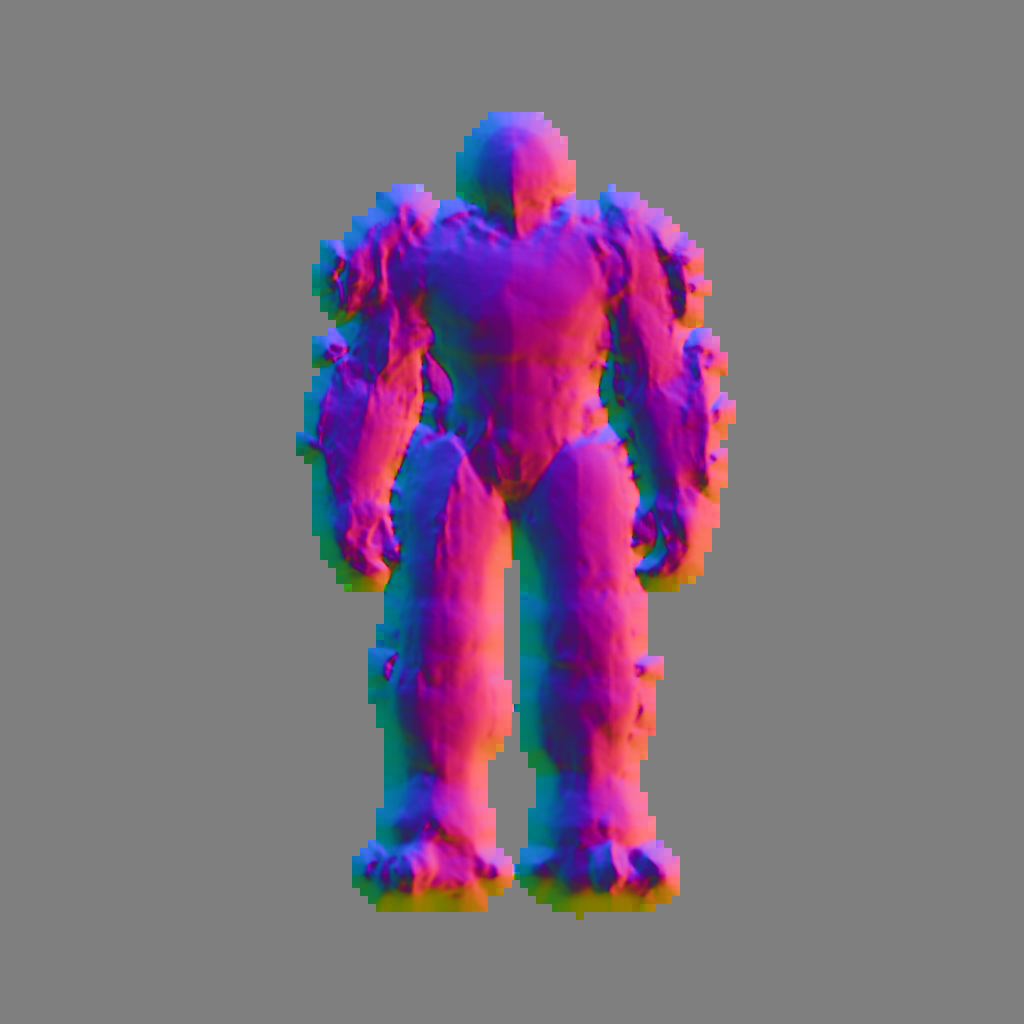
\includegraphics[width=\textwidth]{etc/a robot made out of plants/wonder3d/test/wonder3D_10000_front_part4}
        \caption{}
    \end{subfigure}
    \caption{Front view of the Wonder3D generation process. Only minor changes can be seen between initialization and iteration 10000.}~\label{fig:generationWonder3D}
  \end{figure}